\documentclass[a4paper,11pt,hidelinks]{article}
%\usepackage[a-1b]{pdfx}
\usepackage{hyperref}

\usepackage{subfiles}
\usepackage{epsfig}
\usepackage{plain}
\usepackage{setspace}
%\usepackage{minted}
\usepackage{listings}

\usepackage{mdframed}
\usepackage{graphicx}
\usepackage{caption}
\usepackage{color}
\usepackage{amsmath}
\usepackage{amsthm}
\usepackage{amssymb}
\usepackage{amsfonts}
\usepackage{mathabx}
\usepackage{tcolorbox}
\usepackage{multicol}
\usepackage[english]{babel}
\usepackage[left=2cm,right=2cm,top=2cm,bottom=1.8cm]{geometry}
\usepackage{titlesec} 
\usepackage[utf8x]{inputenc} 

\hypersetup{colorlinks=true,urlcolor=blue}

\newtheorem{theorem}{Question}[subsection]
\renewcommand*{\proofname}{Answer}
\addto\captionsenglish{\renewcommand\proofname{Answer}}

\captionsetup{
  justification=centering,
  singlelinecheck=false,
  font=small,labelfont=bf,labelsep=space}

\begin{document}

\pagestyle{plain}

\begingroup

\renewcommand{\cleardoublepage}{}
\renewcommand{\clearpage}{}

\titleformat{\section}
{\normalfont\Large\bfseries}{\thesection}{1em}{}


\renewcommand{\lstlistingname}{Code}%
\renewcommand{\lstlistlistingname}{List of \lstlistingname s}

\definecolor{codeBackground}{rgb}{0.9, 0.9, 0.9}

% Code environment
\lstnewenvironment{code}[1]{
    \mdframed[%
        backgroundcolor=codeBackground,
        shadow=false,
        linecolor=black!40,
        linewidth=2pt,
        topline=false,
        rightline=false,
        leftline=false
    ]%
    \lstset{%
        moredelim=**[is][\color{blue}]{**}{**},
        moredelim=**[is][\color{teal}]{.-}{-.},
        moredelim=**[is][\color{gray}]{||}{||},
        frame=single,
        framerule=0pt,
        basicstyle=\ttfamily,
        keepspaces=true,
        fontadjust=true,
        basewidth=0.5em
    }%
}{% Spacing between and after caption + before end of mdframed
    \vspace{-1em}
    \endmdframed
    \vspace{-0.5em}
    \captionsetup{type=lstlisting}
    \caption{#1}
    \vspace{1.5em}
    \ignorespaces
}

\newpage

\title{Snort exercise}
\author{Offensive Technologies 2021 \\
    Matteo Franzil \texttt{<matteo.franzil@studenti.unitn.it>} \\
    Claudio Facchinetti \texttt{<claudio.facchinetti@studenti.unitn.it>}
    }

\maketitle
\tableofcontents
\newpage

\section{Solution}

\subsection{Topology}

This photo shows the configuration of the nodes.

\begin{figure}[ht!]
    \centering
    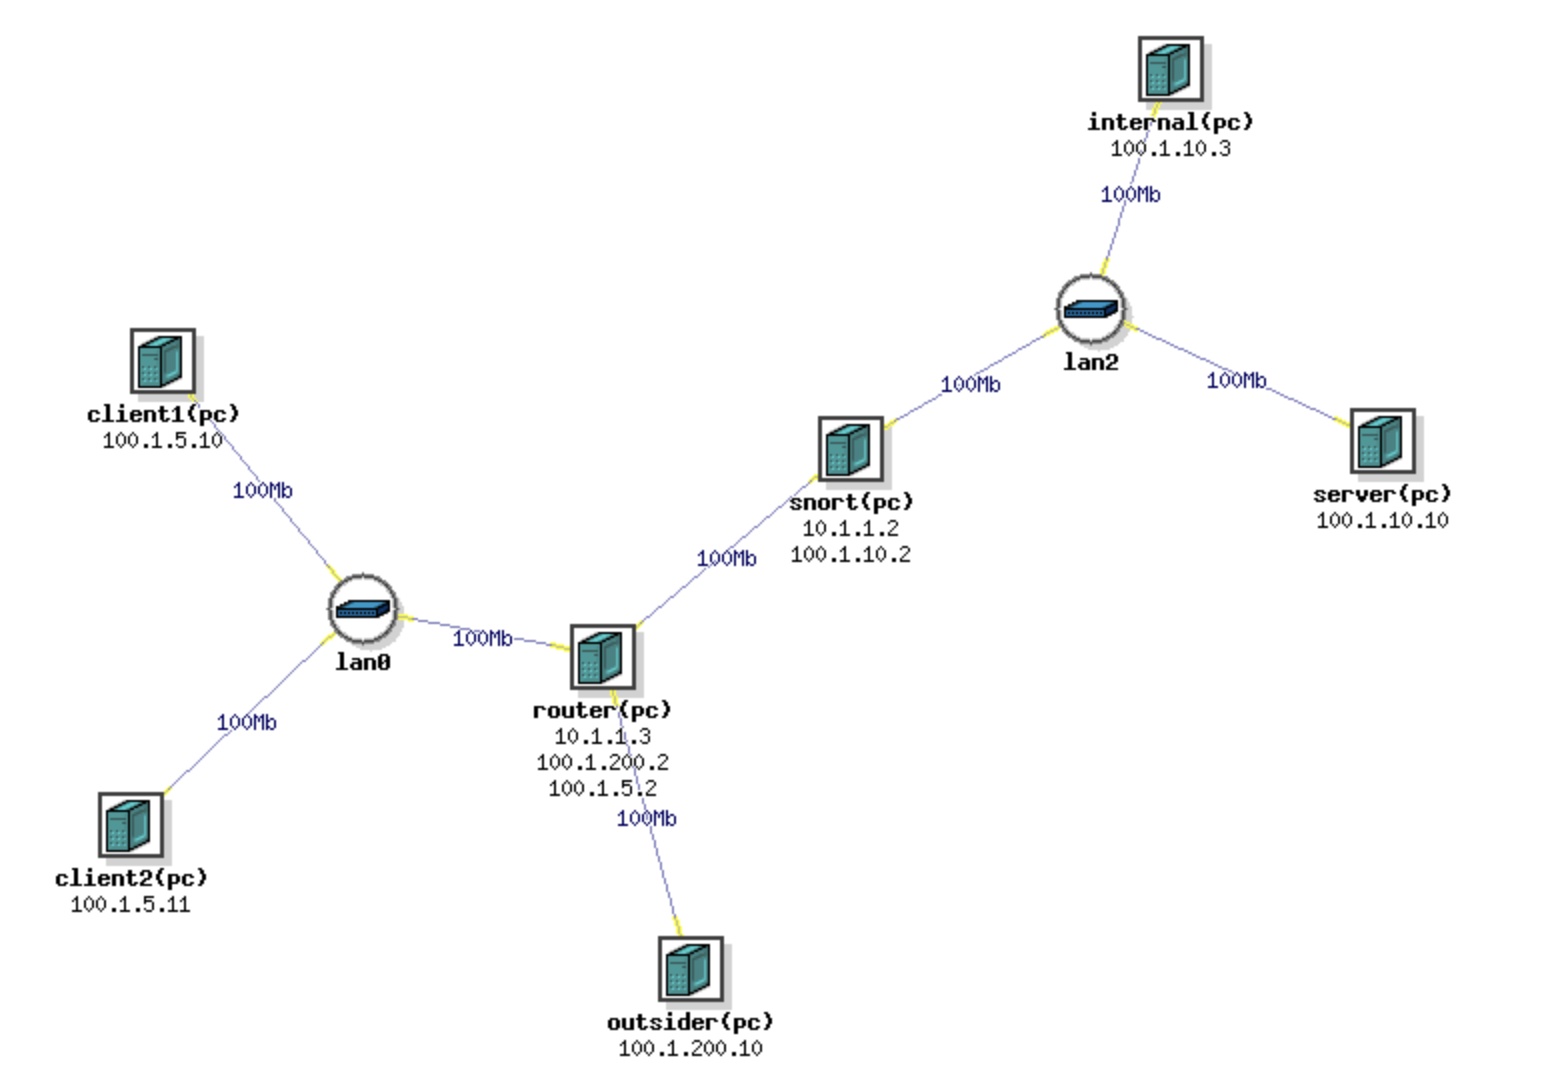
\includegraphics[width=\textwidth]{../drawable/network.png}
    \caption{Network setup for the exercise.}
\end{figure}

\clearpage
\newpage

\subsection{Basic exercises}

\subsubsection{Start Snort Without Rules}

Connect to \verb=users.deterlab.net=. SSH into the \verb=snort= experiment node.

Start Snort without any rules by entering the command \verb=sudo snort --daq nfq -Q -v=. 

Open another terminal and SSH again into \verb=users.deterlab.net= and the \verb=snort= node. In this terminal run \verb=tcpdump= to capture the data going to and from the \verb=client1=. This should be on the interface with an IP Address in the \verb=10.1.1.0/24= range. 

You can run tcpdump using the command:

\begin{code}{Code for using tcpdump}
**# tcpdump -i [interface] -s 0 -w /tmp/dump.pcap**
\end{code}
    
Allow this to run for 30 seconds and then tcpdump by pressing \verb=^C=. Let the Snort process continue running. Now run

\begin{code}{Processing the obtained data.}
**# /share/education/SecuringLegacySystems_JHU/process.pl /tmp/dump.pcap**
\end{code}

This will produce a set of $x,y$ coordinates where $x$ is time and $y$ is number of packets in that second.

\begin{theorem}
    Respond to the following points. 
    \begin{enumerate}
        \item What happens to the traffic to client1 when Snort is not running?
        \item Is this a good thing?
        \item Based on Snort's output what can you say about the application? What port does it connect to?
        \item Please attach a graph of the traffic over time to your answers
        \item What does the "-Q" option do in Snort?
        \item What does the "--daq nfq" option do in Snort?    
    \end{enumerate}
\end{theorem}

\begin{proof}
    These are the answers.
    \begin{enumerate}
        \item When Snort is not running, all traffic gets dropped. We can see a slew of \verb=SYN= packets being continuously sent by clients.
        \item Not really. We can see that there are \verb=client1=, \verb=client2= and \verb=outsider= that are continuously sending traffic to \verb=server=, but it also gets dropped when Snort is not running. Since Snort is working in inline mode, all traffic is supposed to pass through the Snort bridge. When Snort is shut down, then the bridge is left hanging and traffic is automatically dropped.
        \item The application accepts incoming connections on port \verb=7777=.
        \item See the graph at the end of the numbered section.
        \item The -Q option tells Snort to process packets in inline mode.
        \item The --daq nfq option tells Snort to use the \verb=nfq= DAQ module.
    \end{enumerate}

    \begin{figure}[ht!]
        \centering
        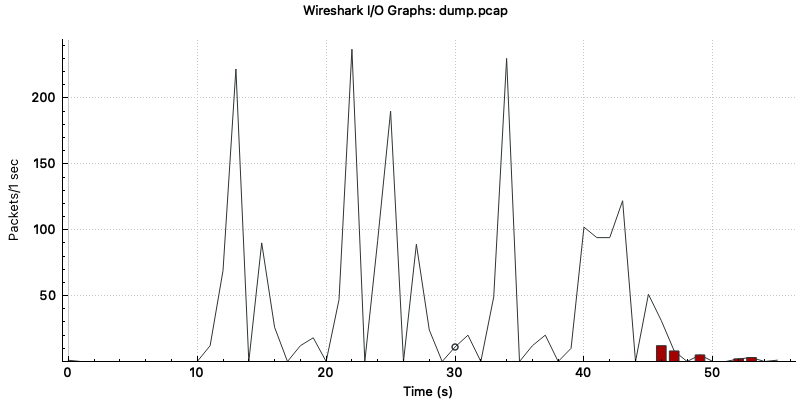
\includegraphics[width=\textwidth]{../drawable/traffic.png}
        \caption{Traffic over time.}
    \end{figure}

\end{proof}

\clearpage

\subsubsection{Analyze Network Traffic}

Connect to the \verb=router= node. Use \verb=ifconfig= to determine which network interfaces connect to which network. Run \verb=tcpdump= to capture the data going to the server. This should be on the interface with an IP Address in the \verb=10.0.1.0/24= range. 

You can run tcpdump with the same command as in Part 1. Let this run for around a minute before terminating it by pressing \verb=^C=. Copy this data to your computer via SCP and open it using Wireshark. 

\begin{theorem}
    Respond to the following points.
    \begin{enumerate}
        \item The request that the client sends the server is broken into four parts. What are these parts and what order does they appear in? How are these parts separated in the request?
        \item Is this is a secure way for the client to send requests to the server? Explain your answer.
        \item Can you recover one of the files sent by the server to a client? If so attach the file, a pcap the relevant packets and indicate which client this was sent to.
    \end{enumerate}
\end{theorem}

\begin{proof}
    These are the answers.
    \begin{enumerate}
        \item Figure \ref{fig:network} shows a snippet of the traffic. In our observations, each of the five different requests that the clients use a particular four-part string protocol in which the data is divided with the \verb=!:.:!= separator. In particular, the first field contains a username, the second contains a password, the third contains the name of the file, the fourth is the actual content of the file preceded by a certain amount of \textit{junk}.
        \item It is not. Disregarding the fact that the connection is not encrypted - so all the payload is in clear and can be easily read with some simple traffic sniffing - the third field contains the name of the file that is attached to the message. This easily allows network sniffers such as Snort to intercept and block such requests if they contain sensitive data, without resorting to file parsing. However, this also allows man-in-the-middle attackers to obtain information about what the client is querying before the data is even retrieved.
        \item See the attached \verb=pcap= file and Figure \ref{fig:follow}. After selecting TCP stream 56, I used the \textit{Follow TCP Stream} Wireshark tool to visualize the data exchanged between the client and the server.
    \end{enumerate}
    
    \begin{figure}[ht!]
        \centering
        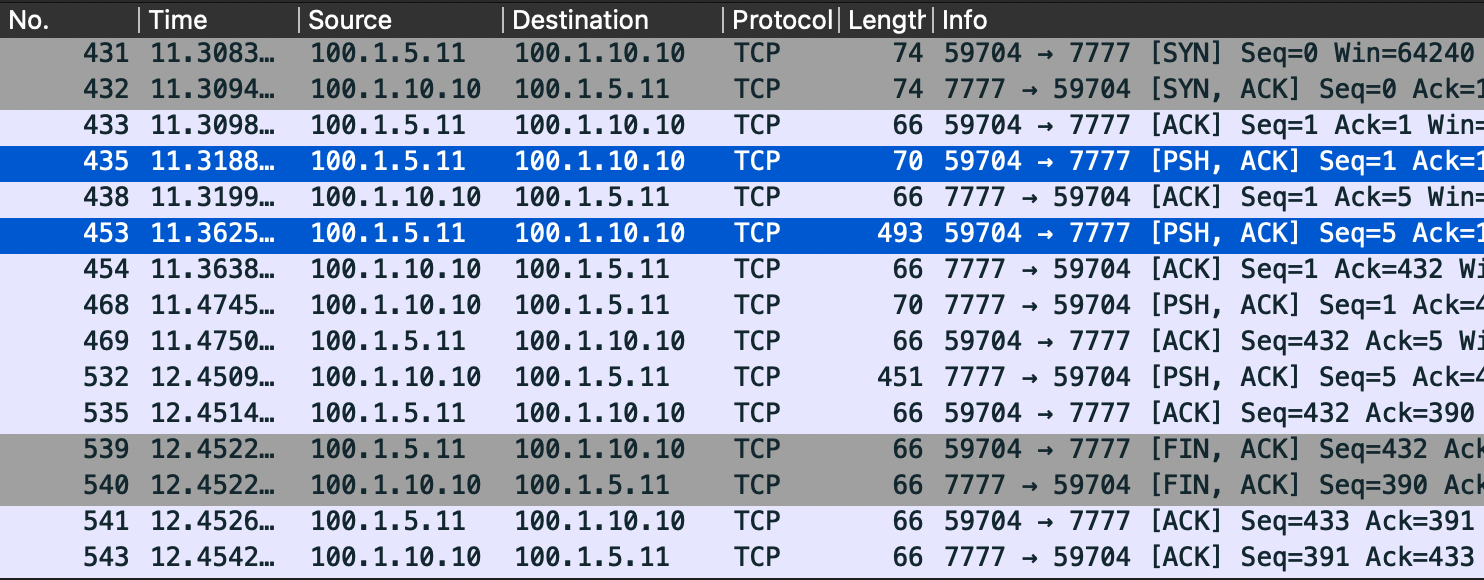
\includegraphics[width=0.8\textwidth]{../drawable/request.png}
        \caption{Snippet of a TCP stream from the first point.}
        \label{fig:network}
    \end{figure}
    
    \begin{figure}[ht!]
        \centering
        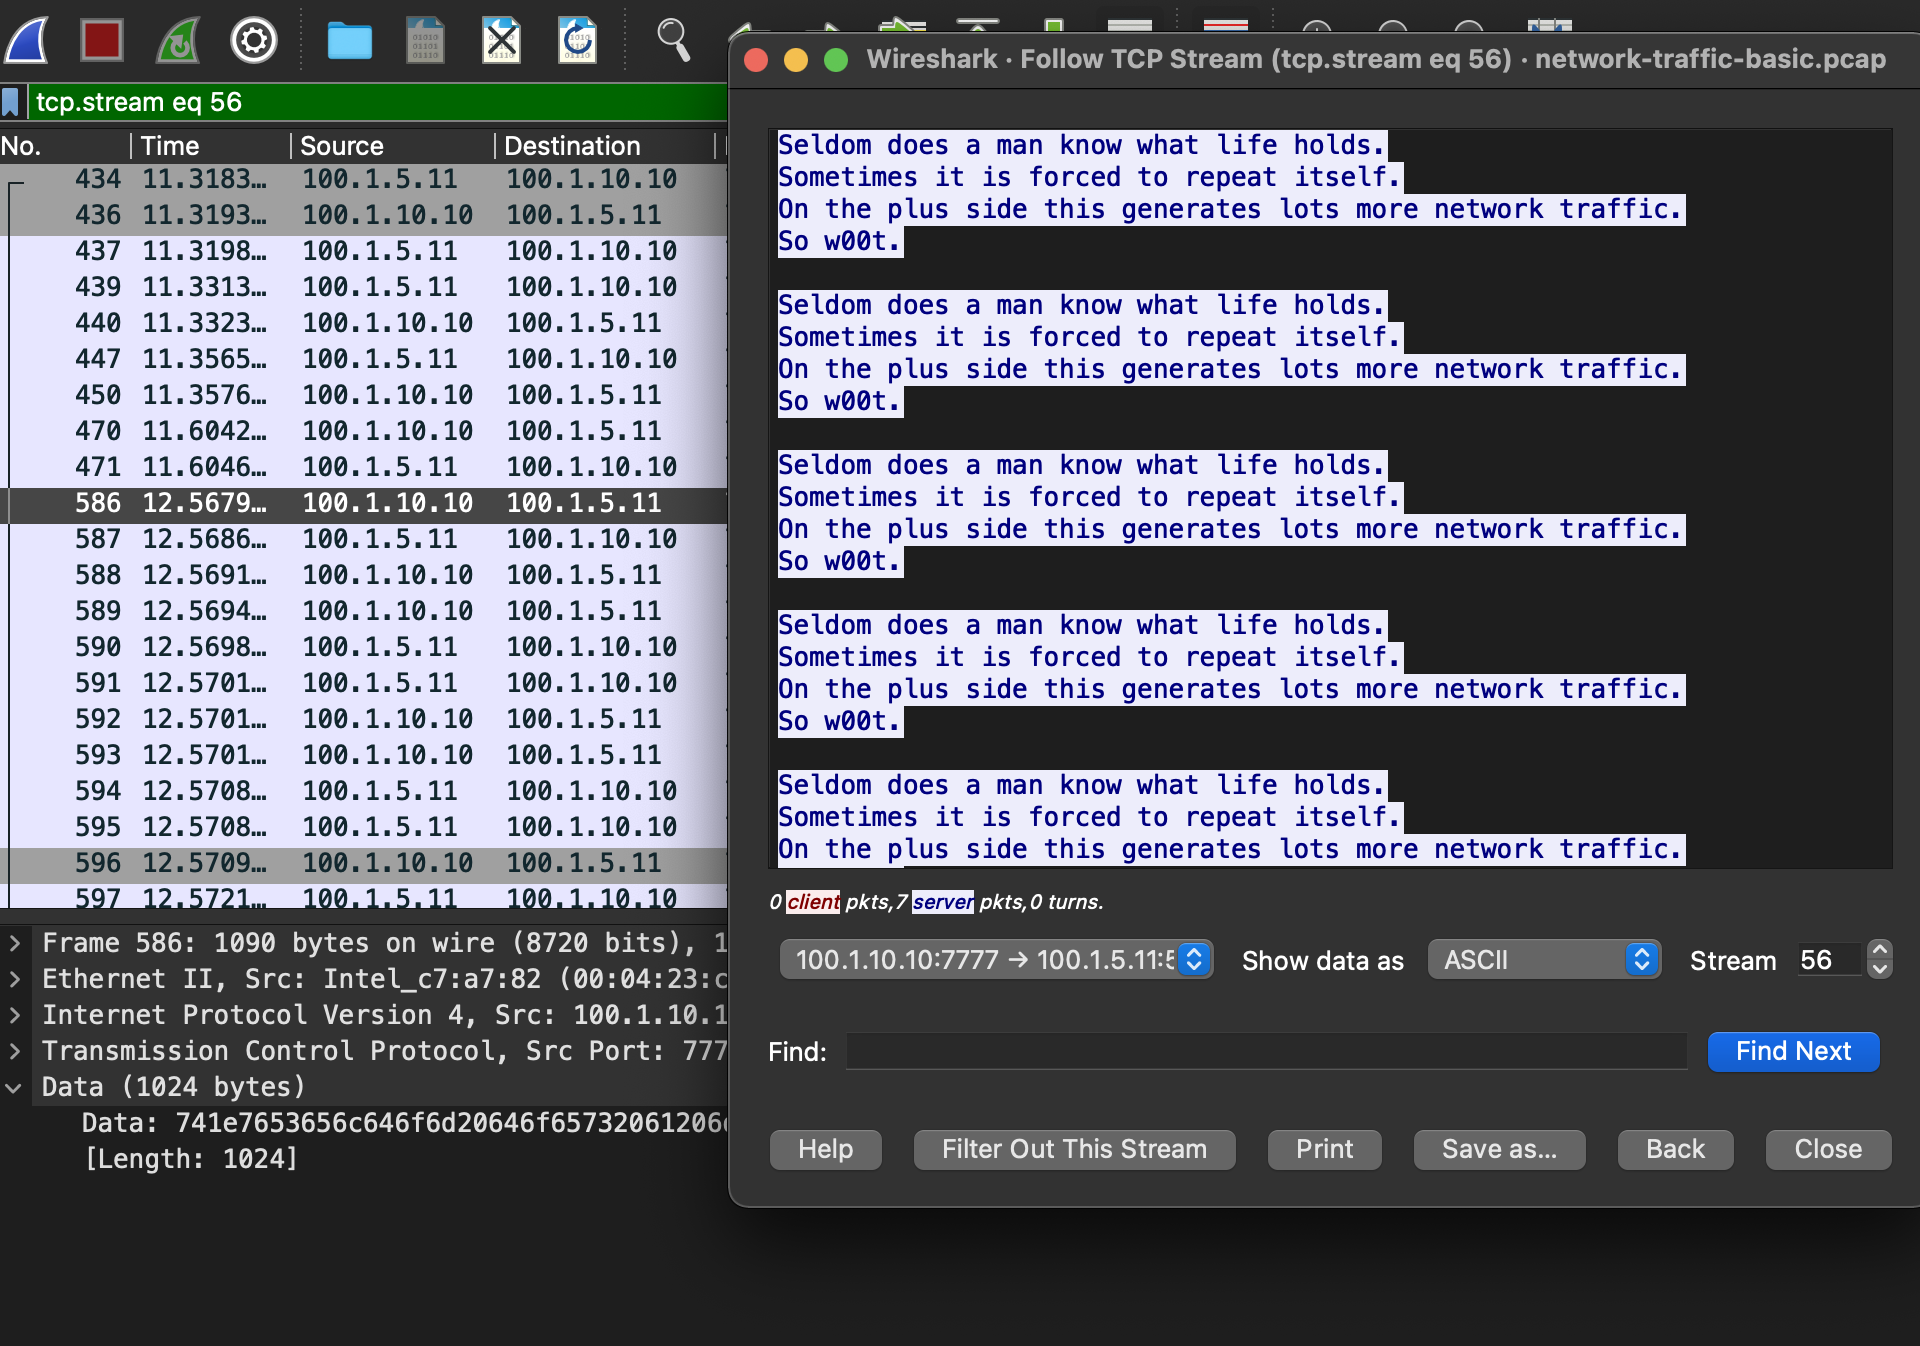
\includegraphics[width=0.8\textwidth]{../drawable/follow-stream.png}
        \caption{Following a TCP stream.}
        \label{fig:follow}
    \end{figure}
\end{proof}

\clearpage

\subsubsection{Write Rules to Guard Against Simple Requests}

In that terminal where Snort is running stop it with \verb=^C=. Write a configuration file for Snort using the command, named \verb=snort.config=. Add the following Snort rule that prevents .xml files from being sent out.

\begin{code}{Code to add to the snort.config}
reject tcp 100.1.0.0/16 ANY -> 100.1.10.10 [Port from Question 3]
    (msg: "XML Read Attempt Detected"; sid:1; content:".xml";)
\end{code}

Using this rule as an example write a rule that prevents classified data from being sent to the outsider computer, but does not prevent it from being sent to any other computers. Now you must make a directory for Snort alerts, called \verb=alerts=. Start Snort using your new rule with the command:

\begin{code}{Code to start snort.}
**# snort --daq nfq -Q -c snort.config -l alerts**
\end{code}

Log onto \verb=client1=, \verb=client2= and \verb=outsider= to see if these rules worked. If you aren't sure go to the folder \verb=/home/test= and delete the existing .txt and .xml files then see which ones are recreated. You can also run the program FileClient manually to find out.
Questions:

\begin{theorem}
    Respond to the following points.
    \begin{enumerate}
        \item What rule did you use to secure the "classified" file?
        \item Capture and compare the network traffic for the server when filtering these results using your configuration file and when no file is used. Attach the graph showing packet rate over time for both of these cases to your submission.
        \item Can you think of any others files or extensions that should be filtered against?
    \end{enumerate}
\end{theorem}

\begin{proof}
    These are the answers.
    \begin{enumerate}
        \item \texttt{reject tcp 100.1.200.10 ANY -> 100.1.10.10 7777} \\ \texttt{(msg: "Data Exfiltration"; sid:1; content:"classified";)}
        \item See Figure \ref{fig:rule} and \ref{fig:norule} for the packets graphs. The difference isn't noticeable: after all, we blocked $\frac{1}{5}$ of the traffic coming from one host out of three, so $\frac{1}{15}$ of the total traffic. The graph isn't enough descriptive to appreciate the difference.
        \item By looking at the downloaded documents, \verb=users.txt= looks like a good candidate to be filtered out.
    \end{enumerate}
    
    \begin{figure}[ht!]
        \centering
        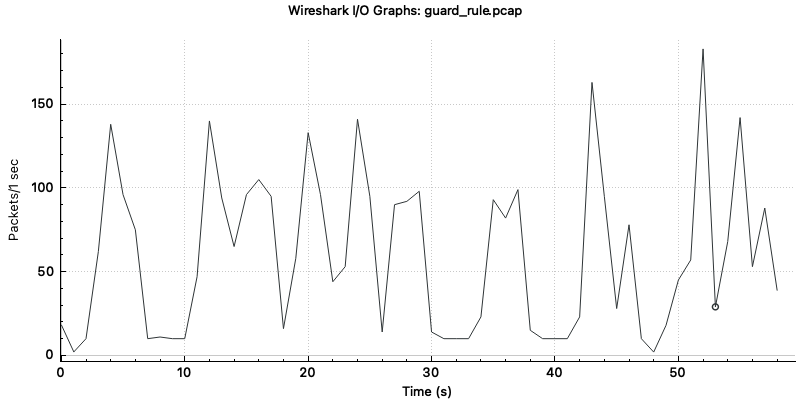
\includegraphics[width=0.7\textwidth]{../drawable/guard_rule.png}
        \caption{Graph of TCP packets with the enabled rule.}
        \label{fig:rule}
    \end{figure}
    
    \begin{figure}[ht!]
        \centering
        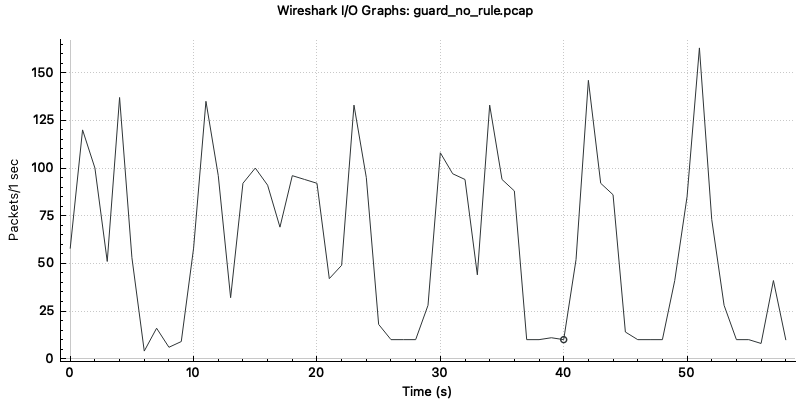
\includegraphics[width=0.7\textwidth]{../drawable/guard_no_rule.png}
        \caption{Graph of TCP packets without the enabled rule.}
        \label{fig:norule}
    \end{figure}
\end{proof}

\clearpage
\newpage

\subsection{Intermediate tasks}

\subsubsection{DOS defense}
\label{subsub:dos}

Connect to the \texttt{server} node and use the \texttt{ip addr} command to find out which is the network interface with the IP address \texttt{100.1.10.10}. Now connect to the \texttt{router} node and use \texttt{ip addr} to determine the network interface which has an IP address in the range \texttt{10.0.1.0/24}.

Run \texttt{tcpdump} on both the \texttt{server} and \texttt{router} nodes on the discovered interfaces to collect traffic when no attack is going on.

Now connect to the \texttt{client1} node and run the following script for 100 seconds to simulate the attack.

\begin{code}{Command to start the attack}
#!/bin/sh
/share/education/TCPSYNFlood_USC_ISI/install-flooder
sudo flooder --src 100.1.5.10 --srcmask 255.255.255.255 --dportmin 7777
    --dportmax 7777 --highrate 100000 --hightime 100
    --dst 100.1.10.10 --dstmask 255.255.255.255
\end{code}

As the attack is ongoing, use again \texttt{tcpdump} to capture traffic on both the \texttt{router} and \texttt{server} machines. Now append the following rules to the \texttt{snort.config} file so that the UDP flooding attack can be avoided.

\begin{code}{Rule for UDP Flooding}
rate_filter gen_id 1, sig_id 10, track by_rule, count 100, 
    seconds 1, new_action drop, timeout 5
event_filter gen_id 1, sig_id 10, track by_rule, count 20,
    seconds 1, type threshold
pass udp any any -> 100.1.10.10/32 7777 (msg: "Possible flooding"; sid: 10;) 
\end{code}

With this rule you are instructing Snort to allow any traffic to the server machine on port 7777; when 100 packets per second are matched then the rate filter starts dropping them. This behaviour remains valid until the threshold imposed by the event filter is higher than the actual number of packets.

Repeat the capturing procedure described above two more times: one with no attack going and one while the attack is active.

\begin{theorem}
    Respond to the following points.
    \begin{enumerate}
        \item Collect the traffic at the server and the router when there is and is not an attack with rules in place that only guard against the attacks mentioned in the basic exercises. Create a graph of this traffic over time.
        \item Repeat the previous step but now with the rate filtering rules enabled.
        \item For a DOS attack should rate filtering rules be paired with event filtering rules?
        \item Try changing the new action in the rate filter to "reject" instead of "drop". What does this do to the traffic and why do you think this is? Is this a good or a bad thing?
        \item Check which interface Snort connects to the router to using \verb=ip addr=. Once you have this information try the above test against while specifying that interface instead of using the default value. This argument will look something like --daq-var device=eth1. Did this change your results. If so attach a graph and explain the change occurred.
        \item Are there any changes you can make outside of Snort to help guard against this attack? If so what are they?
        \item Try running the FileClient program from client2 while this attack is underway. What happens when you have the various rule sets configured?
    \end{enumerate}
\end{theorem}

\begin{proof}
    These are the answers.
    \begin{enumerate}
        \item Graphs can be seen in Section \ref{subsub:graphs}.
        \item Same as before.
        \item Yes, they should always be paired with event filtering rules, otherwise there would be no way of making the new action imposed by the rate limiter revert to the normal behaviour.
        \item When changing the new action to reject instead of drop a RST packet is sent back to the sending machine. If the attacker is not spoofing then nothing bad should happen; if the attacker is spoofing then we might flood the spoofed IP address with a lot of RST packets. In any case changing the behaviour to reject creates more traffic on the network and possibly discloses information, therefore it would be better to stay with drop.
        \item When specified the \texttt{device} variable specifies which interface is used by Snort to capture network traffic. In this case even if we specify the interface connected to the router we would observe little changes: if we make the \texttt{internal} machine use \texttt{snort} as gateway then the only traffic that is no longer captured is the one which from/to the \texttt{internal} node.
        \item Running the FileClient program from the \texttt{client2} node while the attack is in progress results in a higher waiting time before data is received, but it is still able to receive data. The delay is probably caused by the fact that the links are flooded with a high number of packets per second.
    \end{enumerate}
\end{proof}

\subsubsection{DOS defense graphs}
\label{subsub:graphs}

This section shows the graphs requested in the DOS defense exercise (Section \ref{subsub:dos}) .
    
\begin{figure}[ht!]
    \centering
    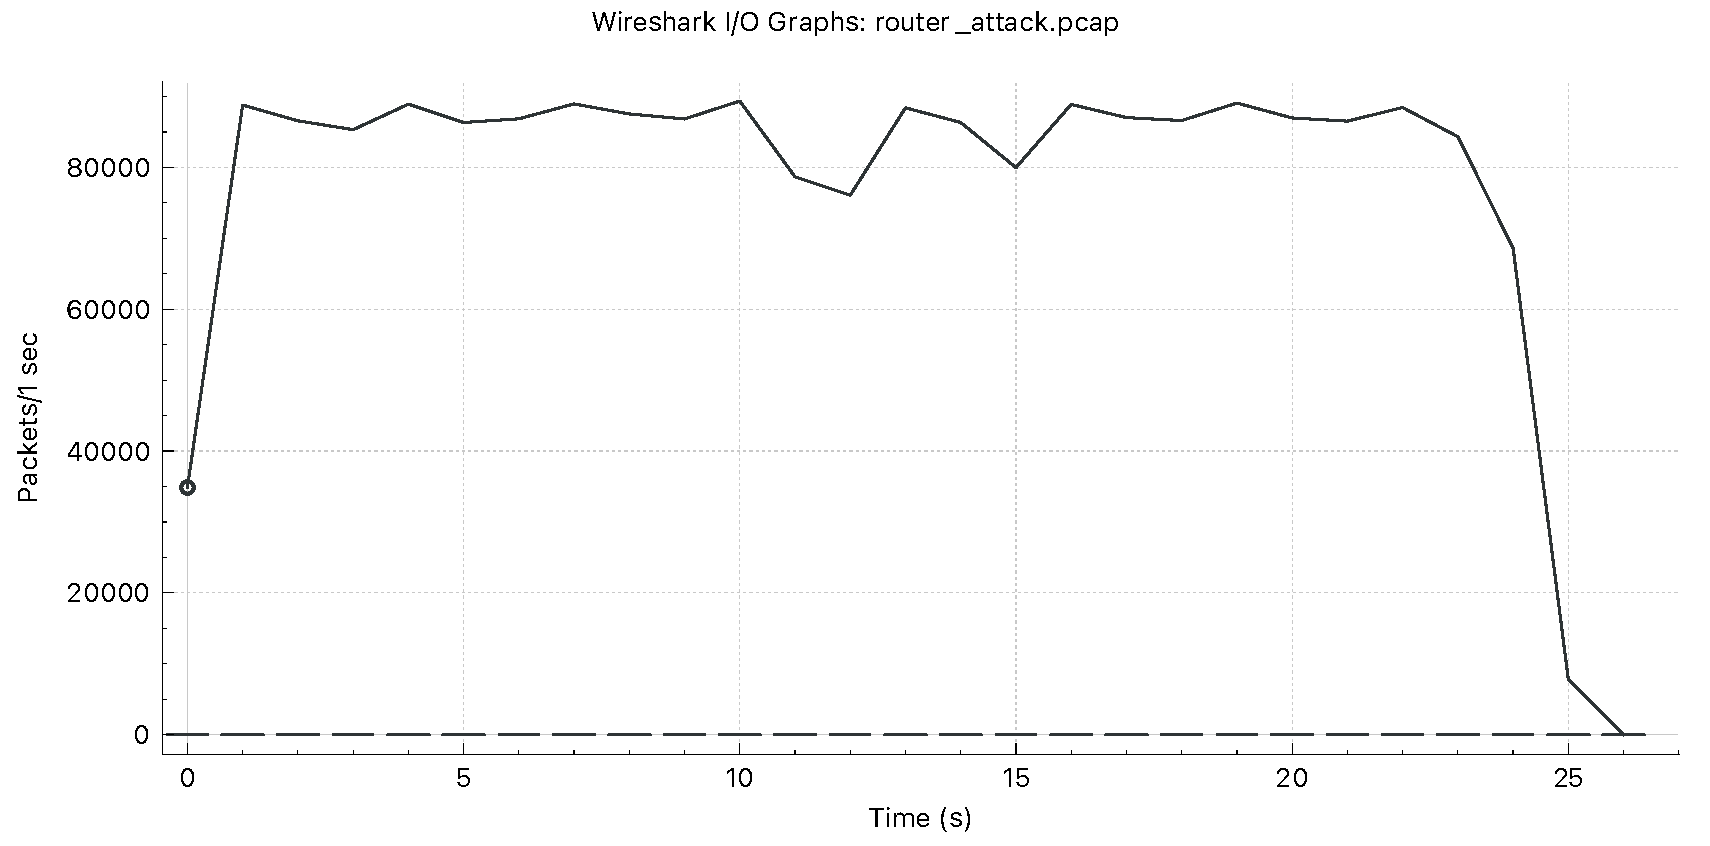
\includegraphics[width=0.4\textwidth]{../drawable/router_attack.pdf}
    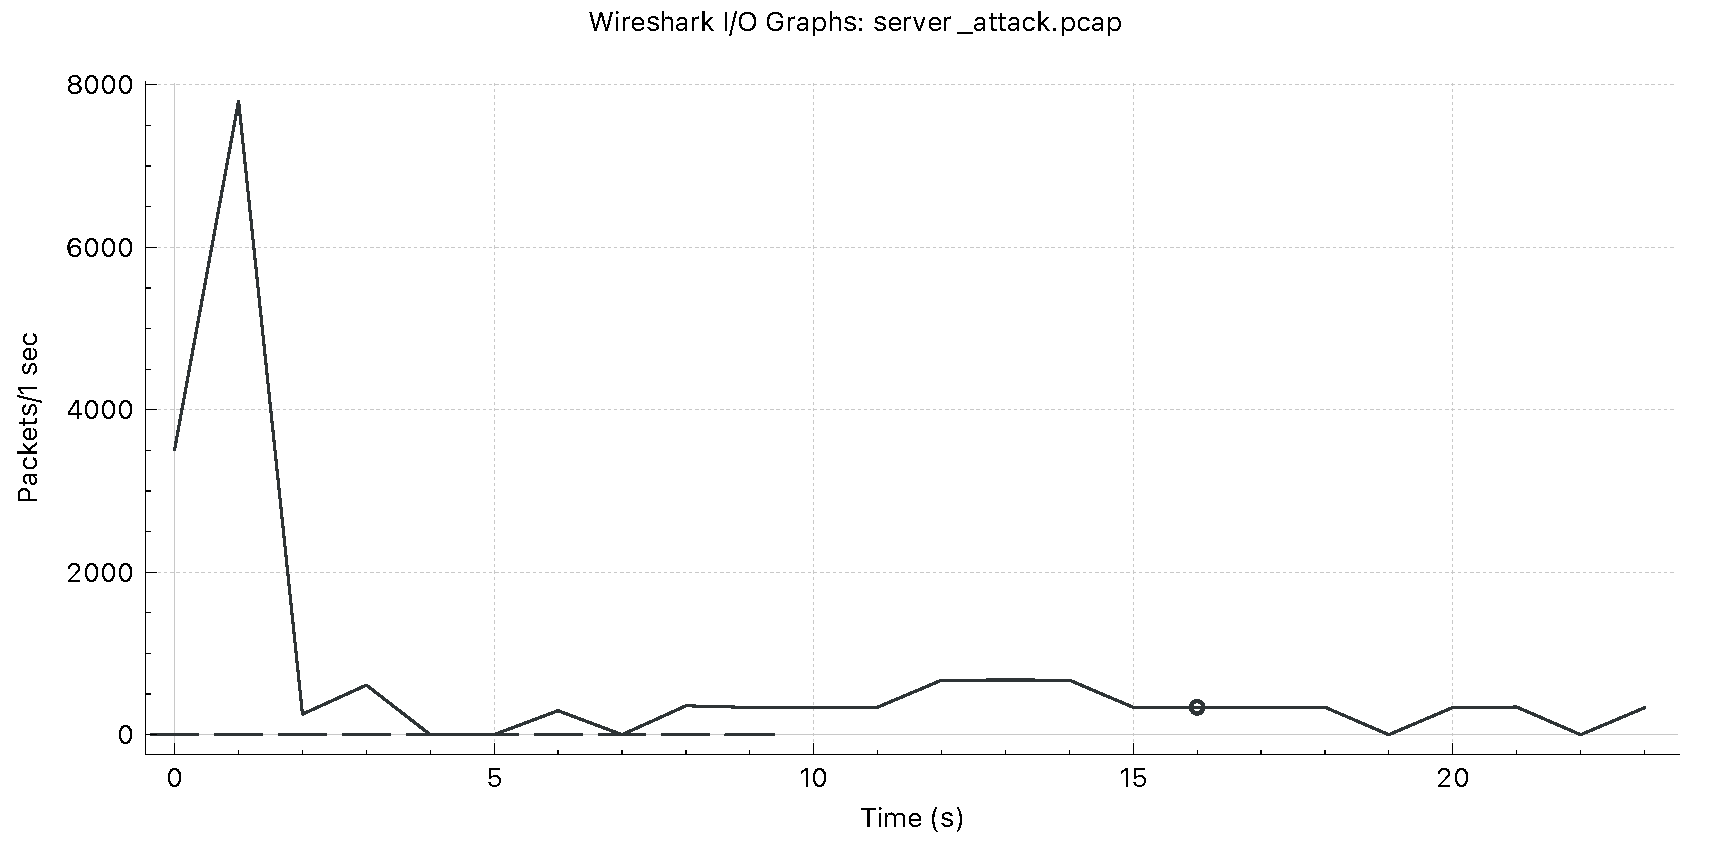
\includegraphics[width=0.4\textwidth]{../drawable/server_attack.pdf}
    \caption{Graph at router and server machines, with \textbf{an attack} ongoing and \textbf{no} rules.}
\end{figure}

\begin{figure}[ht!]
    \centering
    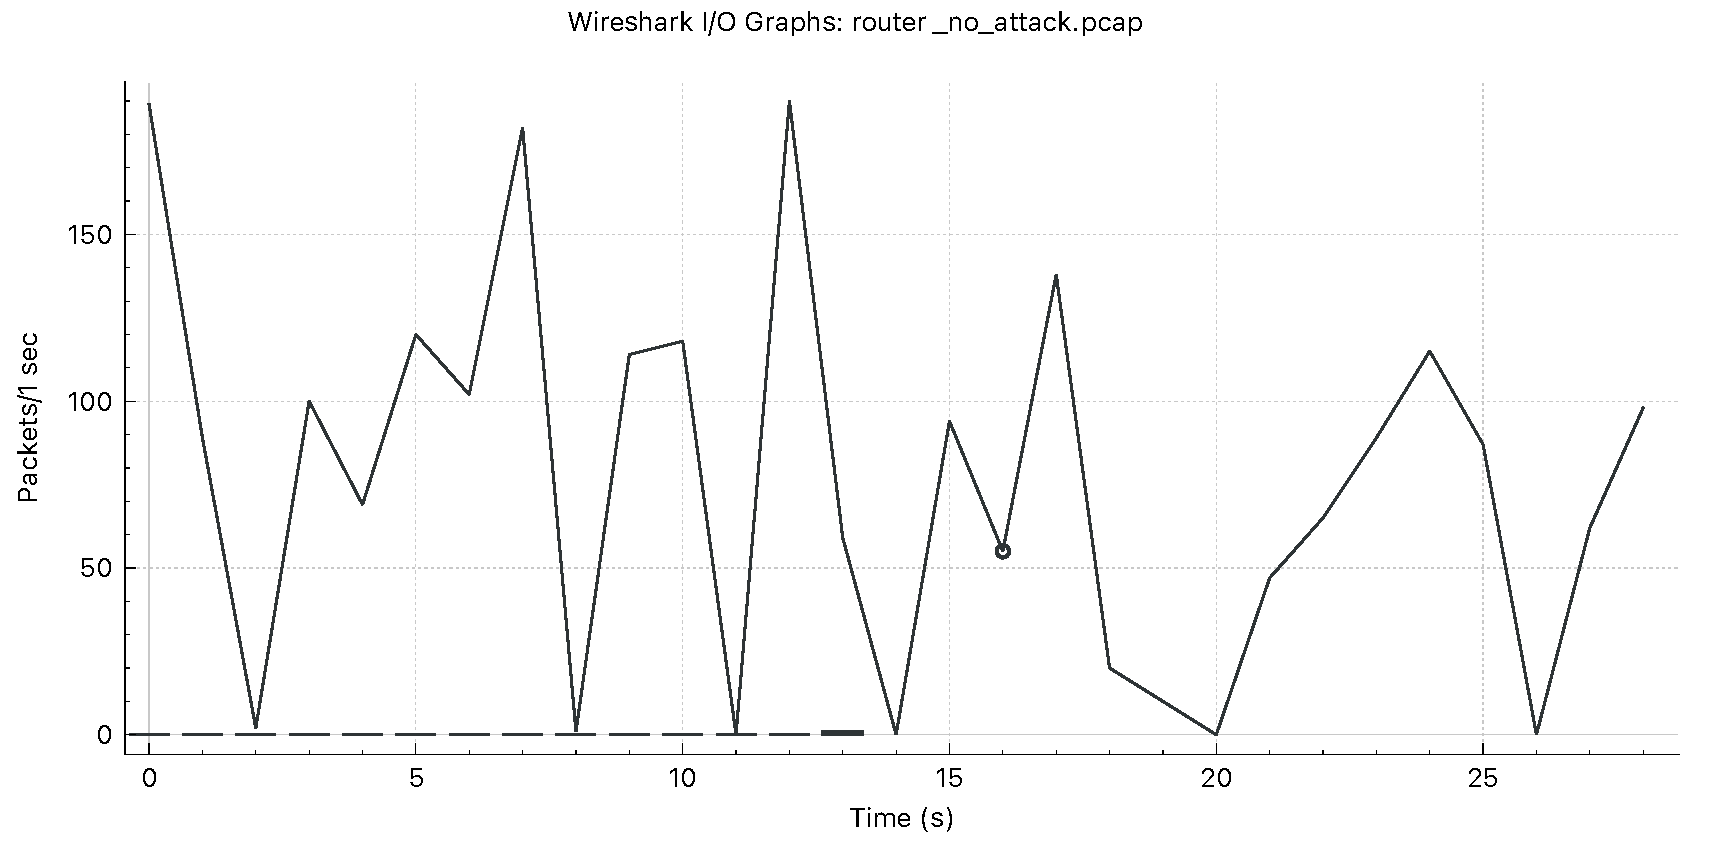
\includegraphics[width=0.4\textwidth]{../drawable/router_no_attack.pdf}
    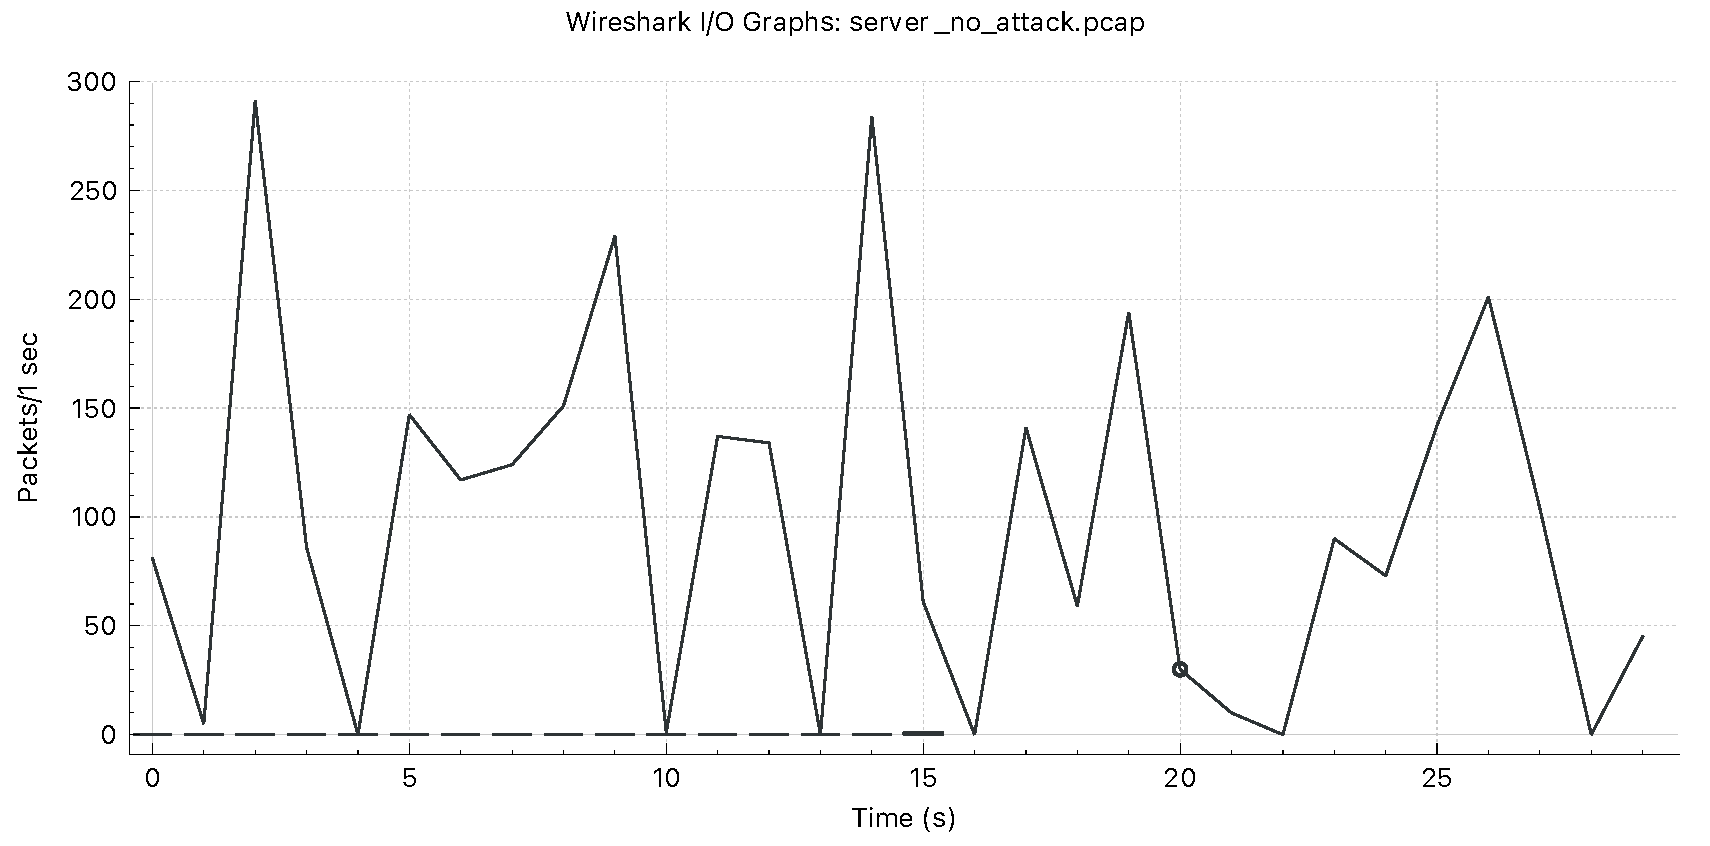
\includegraphics[width=0.4\textwidth]{../drawable/server_no_attack.pdf}
    \caption{Graph at router and server machines, with \textbf{no} attacks ongoing and \textbf{no} rules.}
\end{figure}

\begin{figure}[ht!]
    \centering
    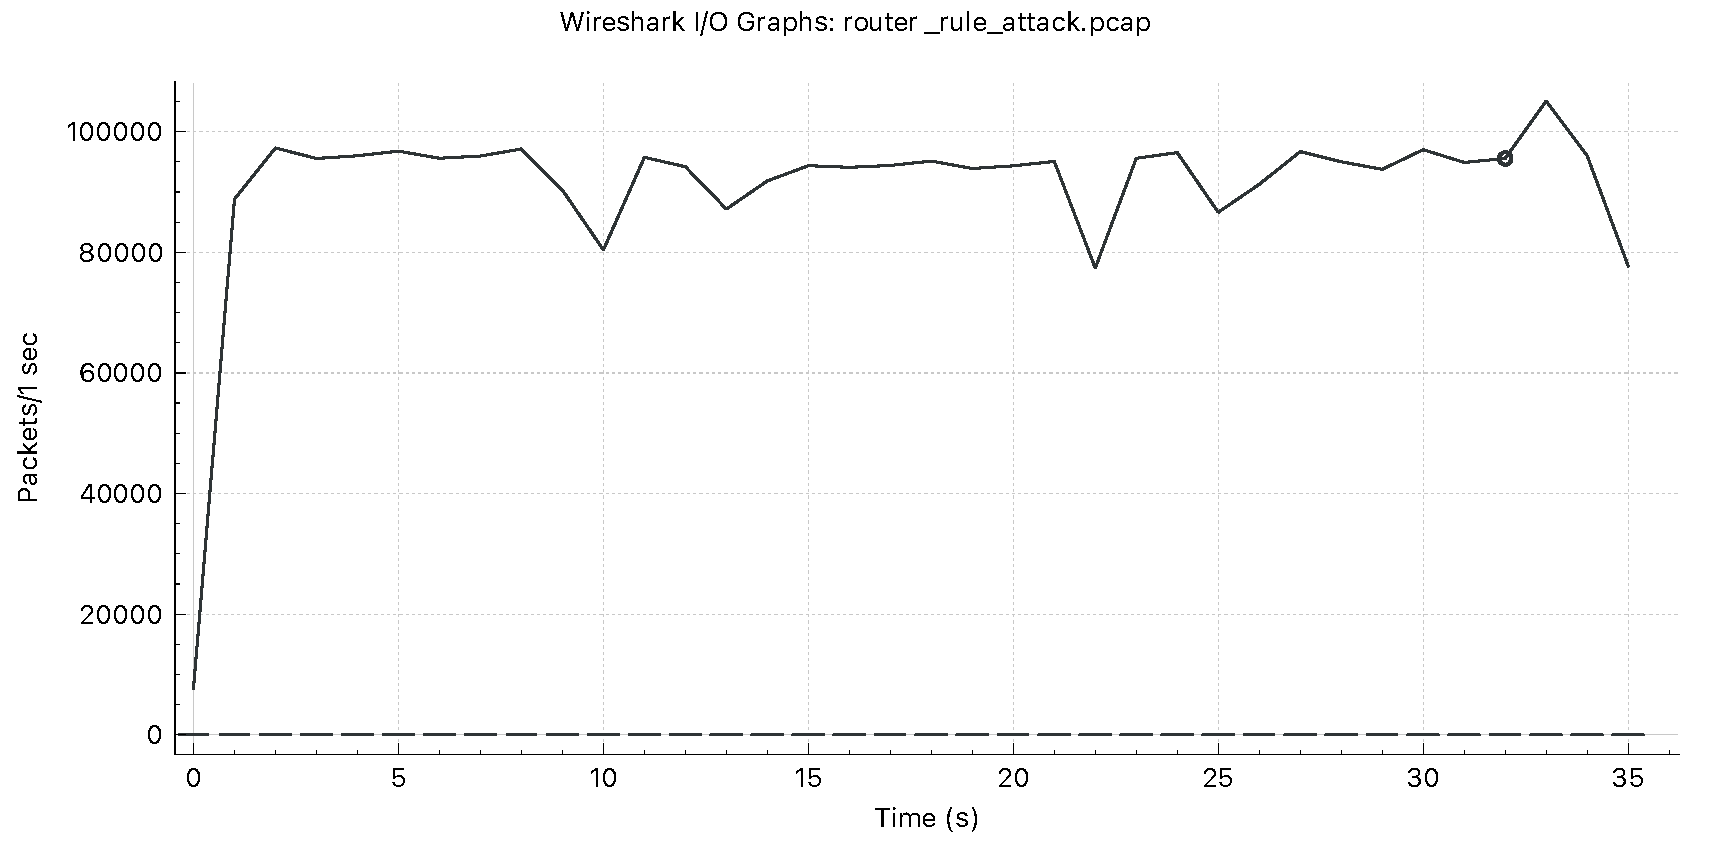
\includegraphics[width=0.4\textwidth]{../drawable/router_rule_attack.pdf}
    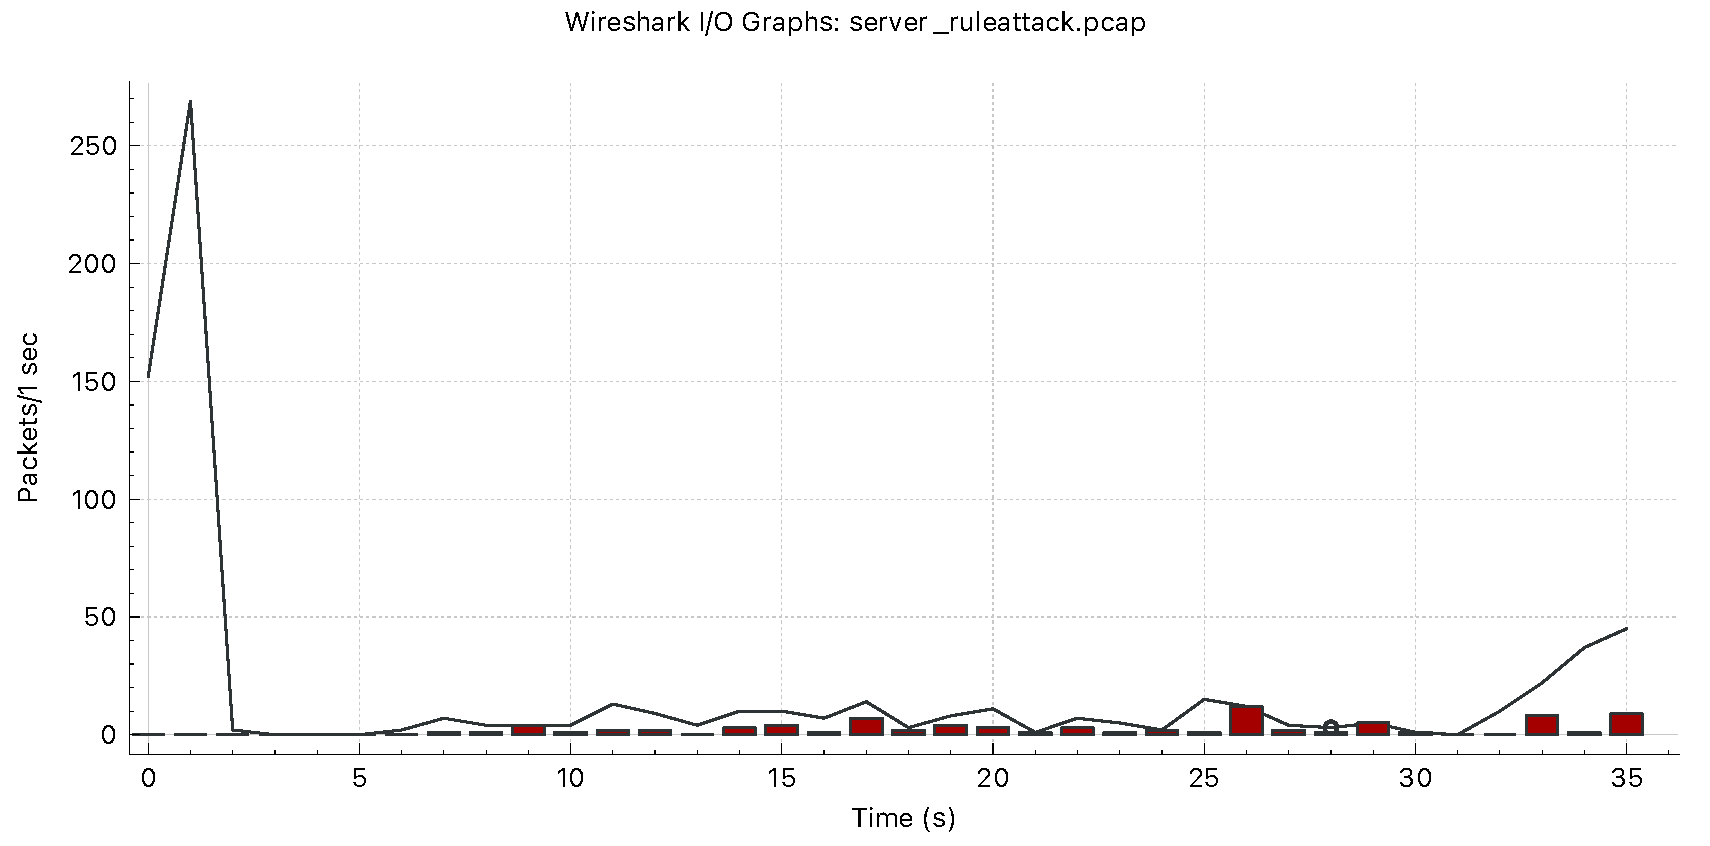
\includegraphics[width=0.4\textwidth]{../drawable/server_rule_attack.pdf}
    \caption{Graph at router and server machines, with \textbf{an attack} ongoing and \textbf{active} rules.}
\end{figure}

\begin{figure}[ht!]
    \centering
    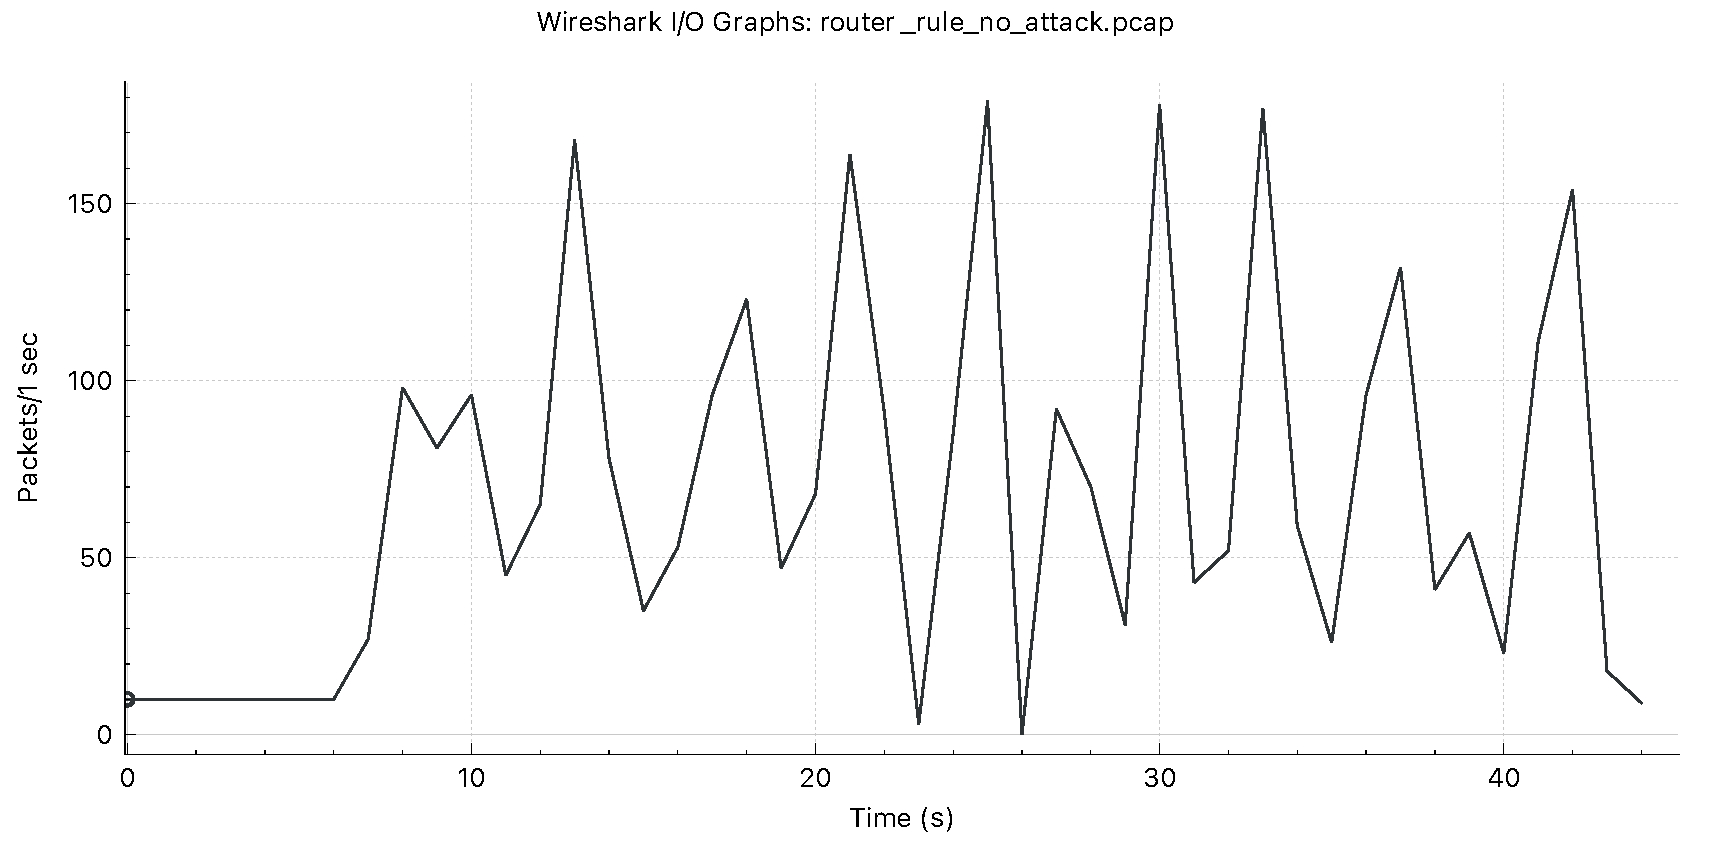
\includegraphics[width=0.4\textwidth]{../drawable/router_rule_no_attack.pdf}
    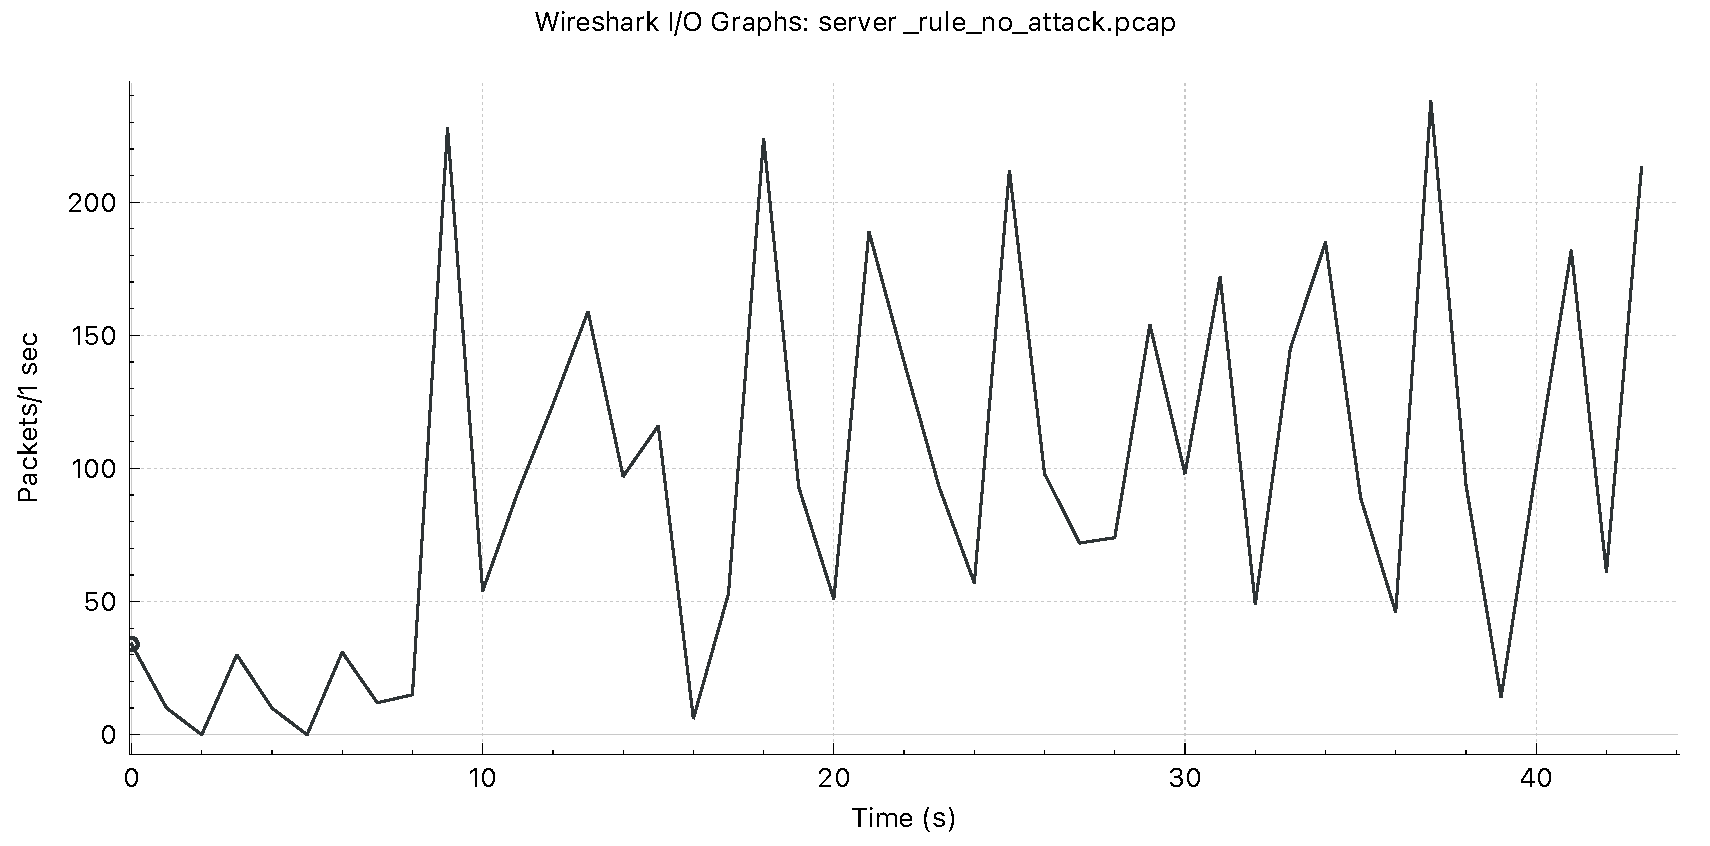
\includegraphics[width=0.4\textwidth]{../drawable/server_rule_no_attack.pdf}
    \caption{Graph at router and server machines, with \textbf{no} attacks ongoing and \textbf{active} rules.}
\end{figure}

\clearpage

\subsubsection{Secure Traffic on the Network}
Connect to the \texttt{internal} machine and run the following command to make the traffic from this machine to the \texttt{server} machine flow through \texttt{snort}.
\begin{code}{Code for replacing the direct route to the server.}
**# route add -host server gw snort**
\end{code}

Verify that the changes had effect by running \texttt{traceroute server} onto the \texttt{internal} machine.

\begin{code}{Result of traceroute on internal machine}
traceroute to server (100.1.10.10), 30 hops max, 60 byte packets
 1  * * *
 2  server-lan2 (100.1.10.10)  0.474 ms  0.477 ms *
\end{code}

\begin{theorem}
    Respond to the following points.
    \begin{enumerate}
        \item Based on the traffic you analyzed what changes could be made to the network to enhance the security of communications coming from client1, client2 and outsider?
        \item What software packages would this require and where should these be installed? Would this cause problems for Snort?
        \item How should the server be configured to prevent internal attacks?
        \item Would this require you to change your Snort configuration in any way?
    \end{enumerate}
\end{theorem}

\begin{proof}
    These are the answers.
    \begin{enumerate}
        \item Right now the communication is completely in plain text and anyone could easily steal usernames and passwords to grab the files. A possible solution to this would be using encryption to secure communications going from client to server and vice versa.
        \item The implementation of cryptography would require some changes to the protocol, meaning that both the client and the server need to be rewritten to support encryption and decryption. This would however be a pain in the neck for Snort: it can no longer check for package content since everything is encrypted and therefore Snort will simply act as a stateful firewall instead of a proper NIDS/NIPS.
        \item In order to be safe against internal attacks the server should require some kind of strong authentication, like physical tokens, in order to perform administrative operations and all the traffic should be filtered through Snort so that there is no traffic left unchecked.
        \item This would probably require some new rules on Snort (blocking potential attacks, allowing protocols, etc) and probably another instance of Snort: if we want to be completely sure an idea could be placing a Snort instance which filters traffic coming from the outside world directed to the internal network and another one which filters intranet traffic. The main idea is that the two instances can have different configurations to prevent different threats. An alternative could be a single instance which filters all the traffic from and to the service, but this would become a single point of failure: if it crashes for any reason the server would be no longer accessible.
    \end{enumerate}
\end{proof}

\clearpage
\newpage

\subsection{Advanced Tasks}
\subsubsection{Code Execution Vulnerability}
As a first thing download from the \texttt{server} machine the file \texttt{FileServer.jar} using the \texttt{scp} util.
\newline
Now install any Java decompiler, such as \texttt{JD-GUI} and open the downloaded file.
\newline
Open the \texttt{jar} file using the Java decompiler and look for a line of code which looks like the one reported below.
\begin{code}{Line causing the code execution}
Runtime.getRuntime.exec(dividedData[2]);
\end{code}
That is the line where it is possible to perform command execution; to do so use the following script one of the client machines. It is fundamental that the payload is at least 2001 characters long.
\begin{code}{Code to shutdown the server remotely}
#!/bin/bash

java -jar FileClient.jar zaqrbo[...]ooob 
    zaqrpassword server sudo%32shutdown%32now
\end{code}

\begin{theorem}
    Respond to the following points.
    \begin{enumerate}
        \item What are the conditions required for this attack to take place?
        \item Create a Snort rule to defend against this attack. You may want to be use pcre instead of content for this rule.
        \item What effect does this rule have on legitimate traffic?
    \end{enumerate}
\end{theorem}

\begin{proof}
    These are the answers.
    \begin{enumerate}
        \item In order to take place the combination of username, password, file name, random junk inserted by the client and separators must be at least 2001 characters long; this string must also contain at least a substring which matches the regular expression \texttt{z.{0,2}a.{0,2}q.{0,2}e}.
        \item In order to defend against this attack append the following rule to the \texttt{snort.config} file.
\begin{code}{Snort rule to defend against RCE}
drop tcp any any -> 100.1.10.10/32 7777
    (msg:"RCE Attempted"; pcre:"/z.{0,2}a.{0,2}q.{0,2}r/"; sid:1000000;)
\end{code}
        \item This rule will block RCE but will also block any legitimate request which will any any username, password, file name or random stuff appended at the end matching that particular regular expression.
    \end{enumerate}
    
    \begin{figure}[ht!]
        \centering
        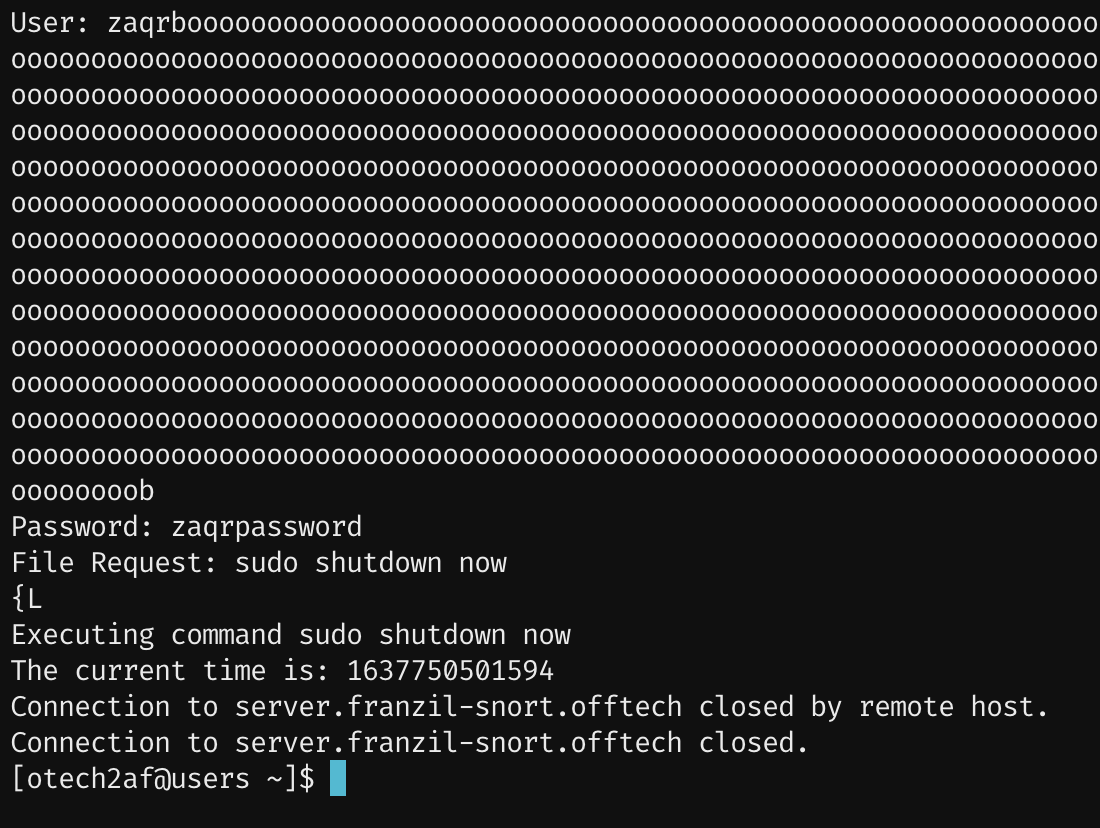
\includegraphics[width=0.66\textwidth]{../drawable/shutdown-tentative.png}
        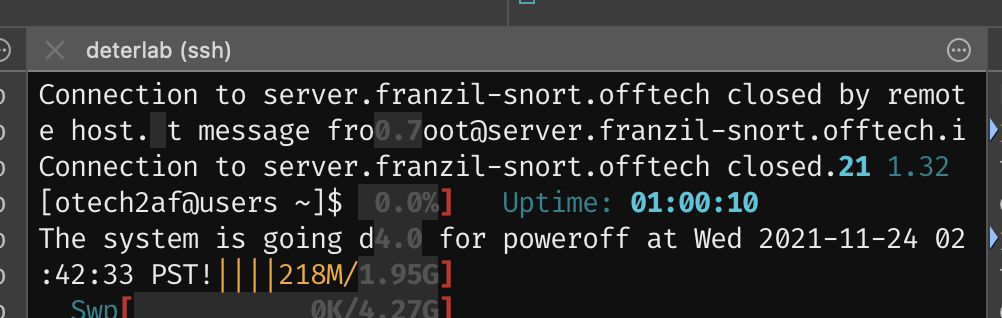
\includegraphics[width=0.66\textwidth]{../drawable/catastrophic-crash.png}
        \caption{Shutting down the server with the exploit.}
    \end{figure}
\end{proof}

\clearpage

\subsubsection{Defend Against ASCII Encoding}

An additional "feature" was recently brought to the attention of the security team: the application has a limited ability to before ASCII decoding. This decoding is triggered whenever the server encounters a \% followed by a number between 0 and 255 at which point the sequence is converted to a single ASCII character.

Now go to the following directory: 
\begin{verbatim}
    /usr/local/snort-2.9.2.2/src/dynamic-examples/dynamic-preprocessor
\end{verbatim}

This contains an example Snort preprocessor. Snort preprocessors allow for advanced data manipulation to normalize data and perform other functions that normal rules cannot. All Snort preprocessors are coded in C. Copy the include folder using the following command:

\begin{code}{Code for including the folder.}
**# cp -rf /usr/local/snort-2.9.2.2/src/dynamic-preprocessors/include/ ..**
\end{code}

You should now be able to compile and install this preprocessor using the command:

\begin{code}{Make command.}
**# make && make install**
\end{code}

Once this has been installed you can use this preprocessor in Snort. To do this edit your configuration file by adding the following lines at the top of the file which tell Snort to auto-generate the decoder rules so you don't have to, the location of the preprocessor library and the preprocessor you wish to use along with all of its arguments (in this case just the port to use):

\begin{code}{Code for adding the preprocessor to the configuration file.}
config autogenerate_preprocessor_decoder_rules
dynamicpreprocessor directory /usr/local/lib/snort_dynamicpreprocessor/
preprocessor dynamic_example: port 7777
\end{code}

Once you have made these changes try to run Snort using your configuration file. At this point it should behave exactly as before, but it now has a preprocessor loaded.

\begin{theorem}
    Respond to the following points.
    \begin{enumerate}
        \item Were you able to bypass your existing rules because of this feature? If so what input strings did you use?
        \item Can you think of a content rule to effectively defend against an attack that uses this feature? Would this affect legitimate traffic?
        \item Snort includes support for user written preprocessors that can render data for Snort's other rules. How would the use of a preprocessor help with this task?
        \item Write a preprocessor to help with this task. Please attach all of the functions you used and the snort.config file that called the preprocessor.
    \end{enumerate}
\end{theorem}

\begin{proof}
    These are the answers.
    \begin{enumerate}
        \item Since \verb=zaqr=, an offending substring in the preivous output, can be encoded as \verb=%122%097%113%114=, then one could do a request such as:
        \begin{verbatim}
java -jar FileClient.jar \
    %122%097%113%114bo[...]b %122%097%113%114password \
    server sudo%32shutdown%32now
        \end{verbatim}
        which would pass through the filters and execute the vulnerability.
    
        \item One idea would be to create a content rule (pcre), with a \% followed by any number, but it would apparently risk being in the way of actual strings containing legitimate \% symbols followed by numbers (e.g. clients visiting files with actual \% characters in the filenames). However, since the server would do the parsing anyway
        \item The preprocessor would be able to parse the payloads of incoming packets, and systematically substitute any \% followed by a number $[0, 255]$ with the corresponding ASCII code. At this point, any malevolent request would be easily spotted and neutralized by the previous rule.
        \item See the attached files. The edited function was the \verb=ExampleProcess= one, which processes packet data before other rules have a chance to access it. 
    \end{enumerate}
\end{proof}

\endgroup
\end{document}